\documentclass[10pt]{beamer}

\usetheme[progressbar=frametitle]{metropolis}
\usepackage{appendixnumberbeamer}

\usepackage{booktabs}
\usepackage[scale=2]{ccicons}

\usepackage{pgfplots}
\usepgfplotslibrary{dateplot}

\usepackage{xspace}
\newcommand{\themename}{\textbf{\textsc{metropolis}}\xspace}

% подключаем кириллицу 
\usepackage[T2A]{fontenc}
\usepackage[utf8]{inputenc}
\usepackage{listings}
\usepackage{graphicx}
\usepackage{hyperref}
\usepackage{chronology}


\title{Metropolis}
\subtitle{A modern beamer theme}
% \date{\today}
\date{}
\author{Matthias Vogelgesang}
\institute{Center for modern beamer themes}
% \titlegraphic{\hfill
\includegraphics[height=1.5cm]{logo.pdf}}





\title{Семинар 2}
\subtitle{Введение в алгоритмы. Хэш-таблицы.}
%\date{\small{\jobname}}
%\date{\today}
\author{\texttt{Бирюков Владимир}}
\institute{МФТИ}



\begin{document}

%-=-=-=-=-=-=-=-=-=-=-=-=-=-=-=-=-=-=-=-=-=-=-=-=
%
%	TITLE PAGE
%
%-=-=-=-=-=-=-=-=-=-=-=-=-=-=-=-=-=-=-=-=-=-=-=-=

\maketitle

%\begin{frame}[plain]
%	\titlepage
%\end{frame}

%-=-=-=-=-=-=-=-=-=-=-=-=-=-=-=-=-=-=-=-=-=-=-=-=
%
%	TABLE OF CONTENTS: OVERVIEW
%
%-=-=-=-=-=-=-=-=-=-=-=-=-=-=-=-=-=-=-=-=-=-=-=-=

\section{Хэш-таблицы}

%-=-=-=-=-=-=-=-=-=-=-=-=-=-=-=-=-=-=-=-=-=-=-=-=
%	TM: AT and definition
%-=-=-=-=-=-=-=-=-=-=-=-=-=-=-=-=-=-=-=-=-=-=-=-=

\begin{frame}{Хэш-таблица.}
\begin{figure}
\centerline{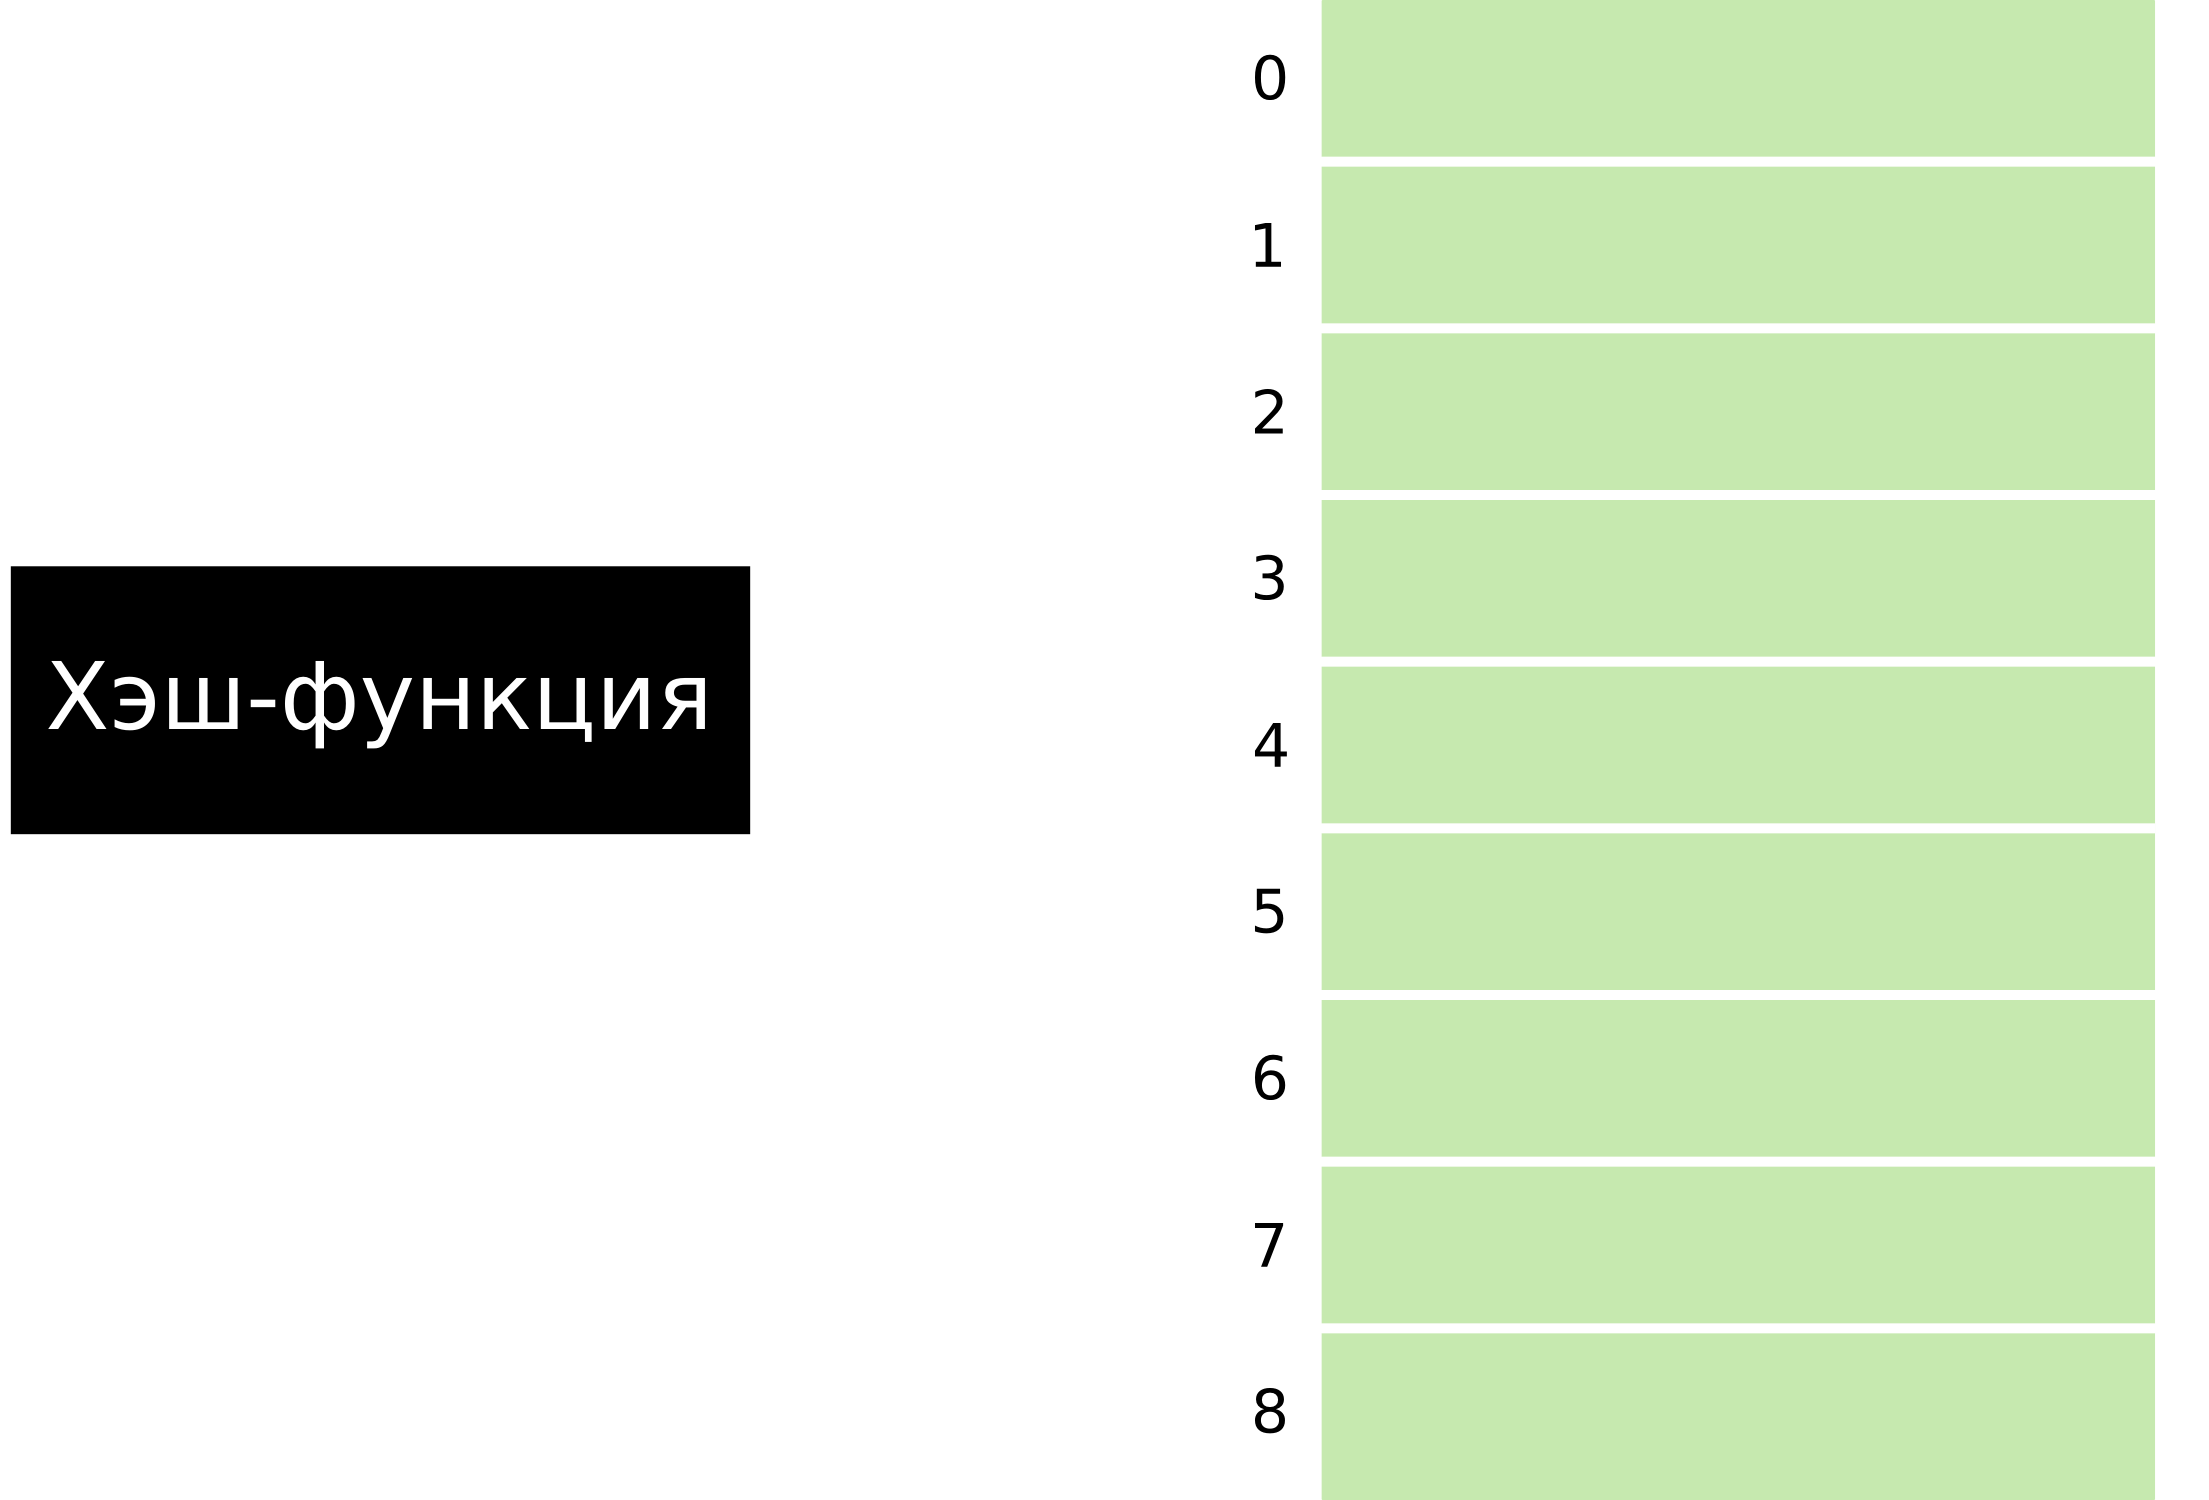
\includegraphics[width=0.86\linewidth]{images/hash_1.png}}
\end{figure}
\end{frame}

\begin{frame}{Хэш-таблица.}
\begin{figure}
\centerline{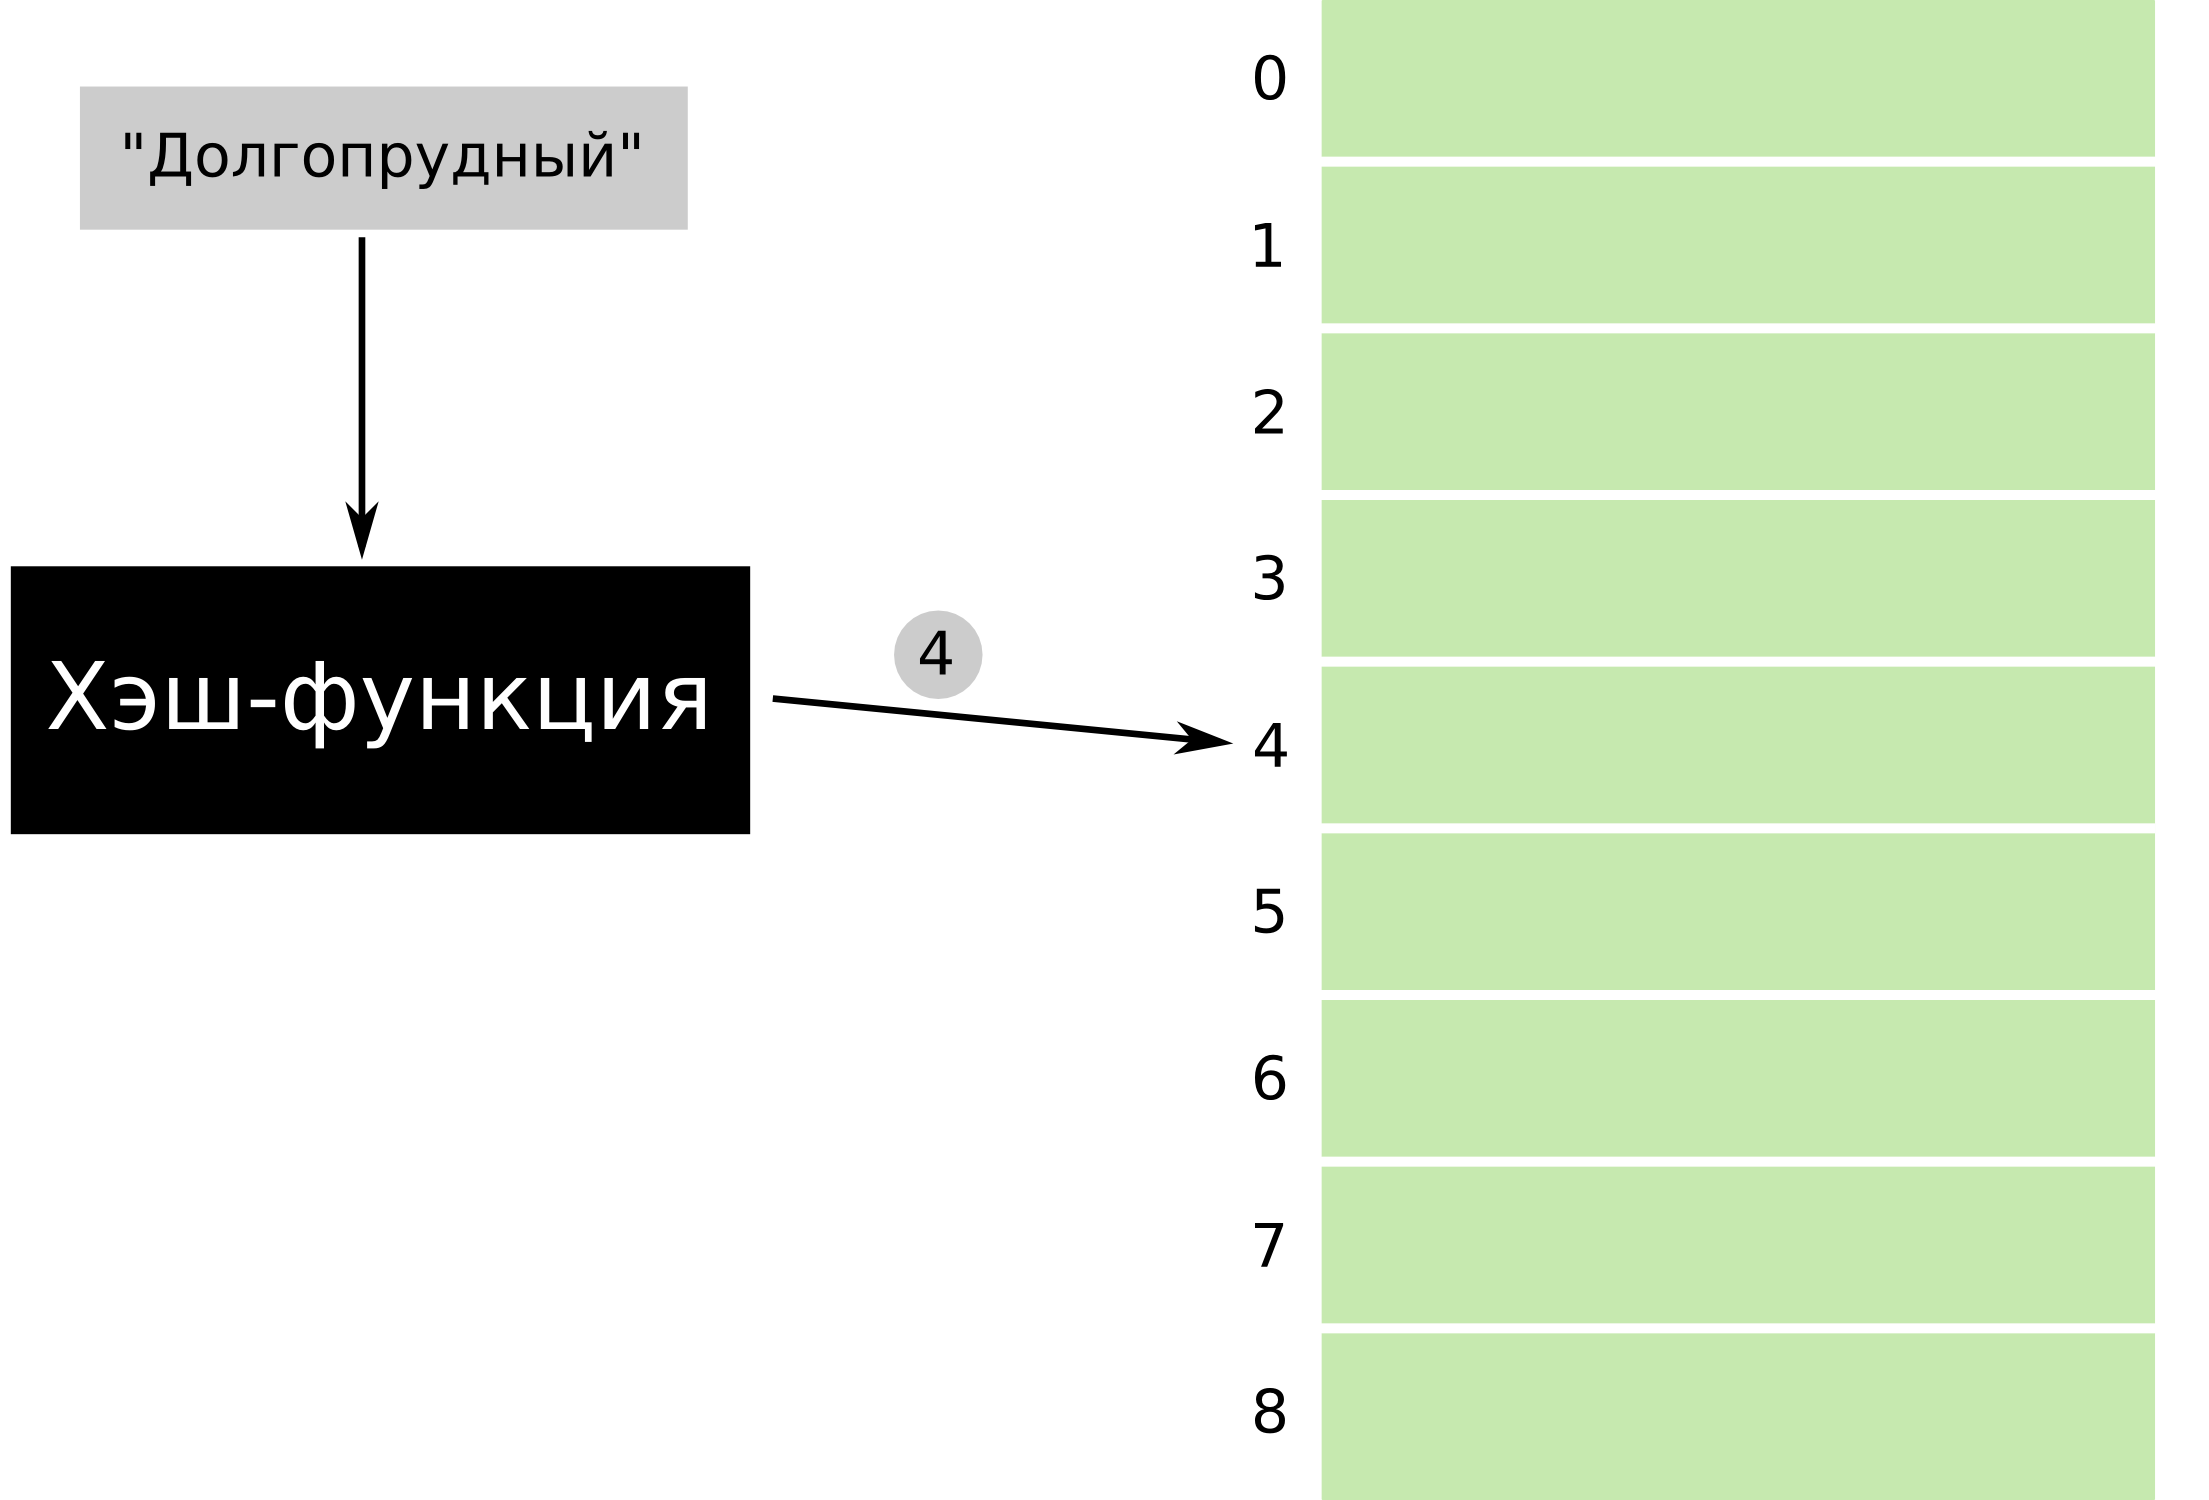
\includegraphics[width=0.86\linewidth]{images/hash_2.png}}
\end{figure}
\end{frame}

\begin{frame}{Хэш-таблица.}
\begin{figure}
\centerline{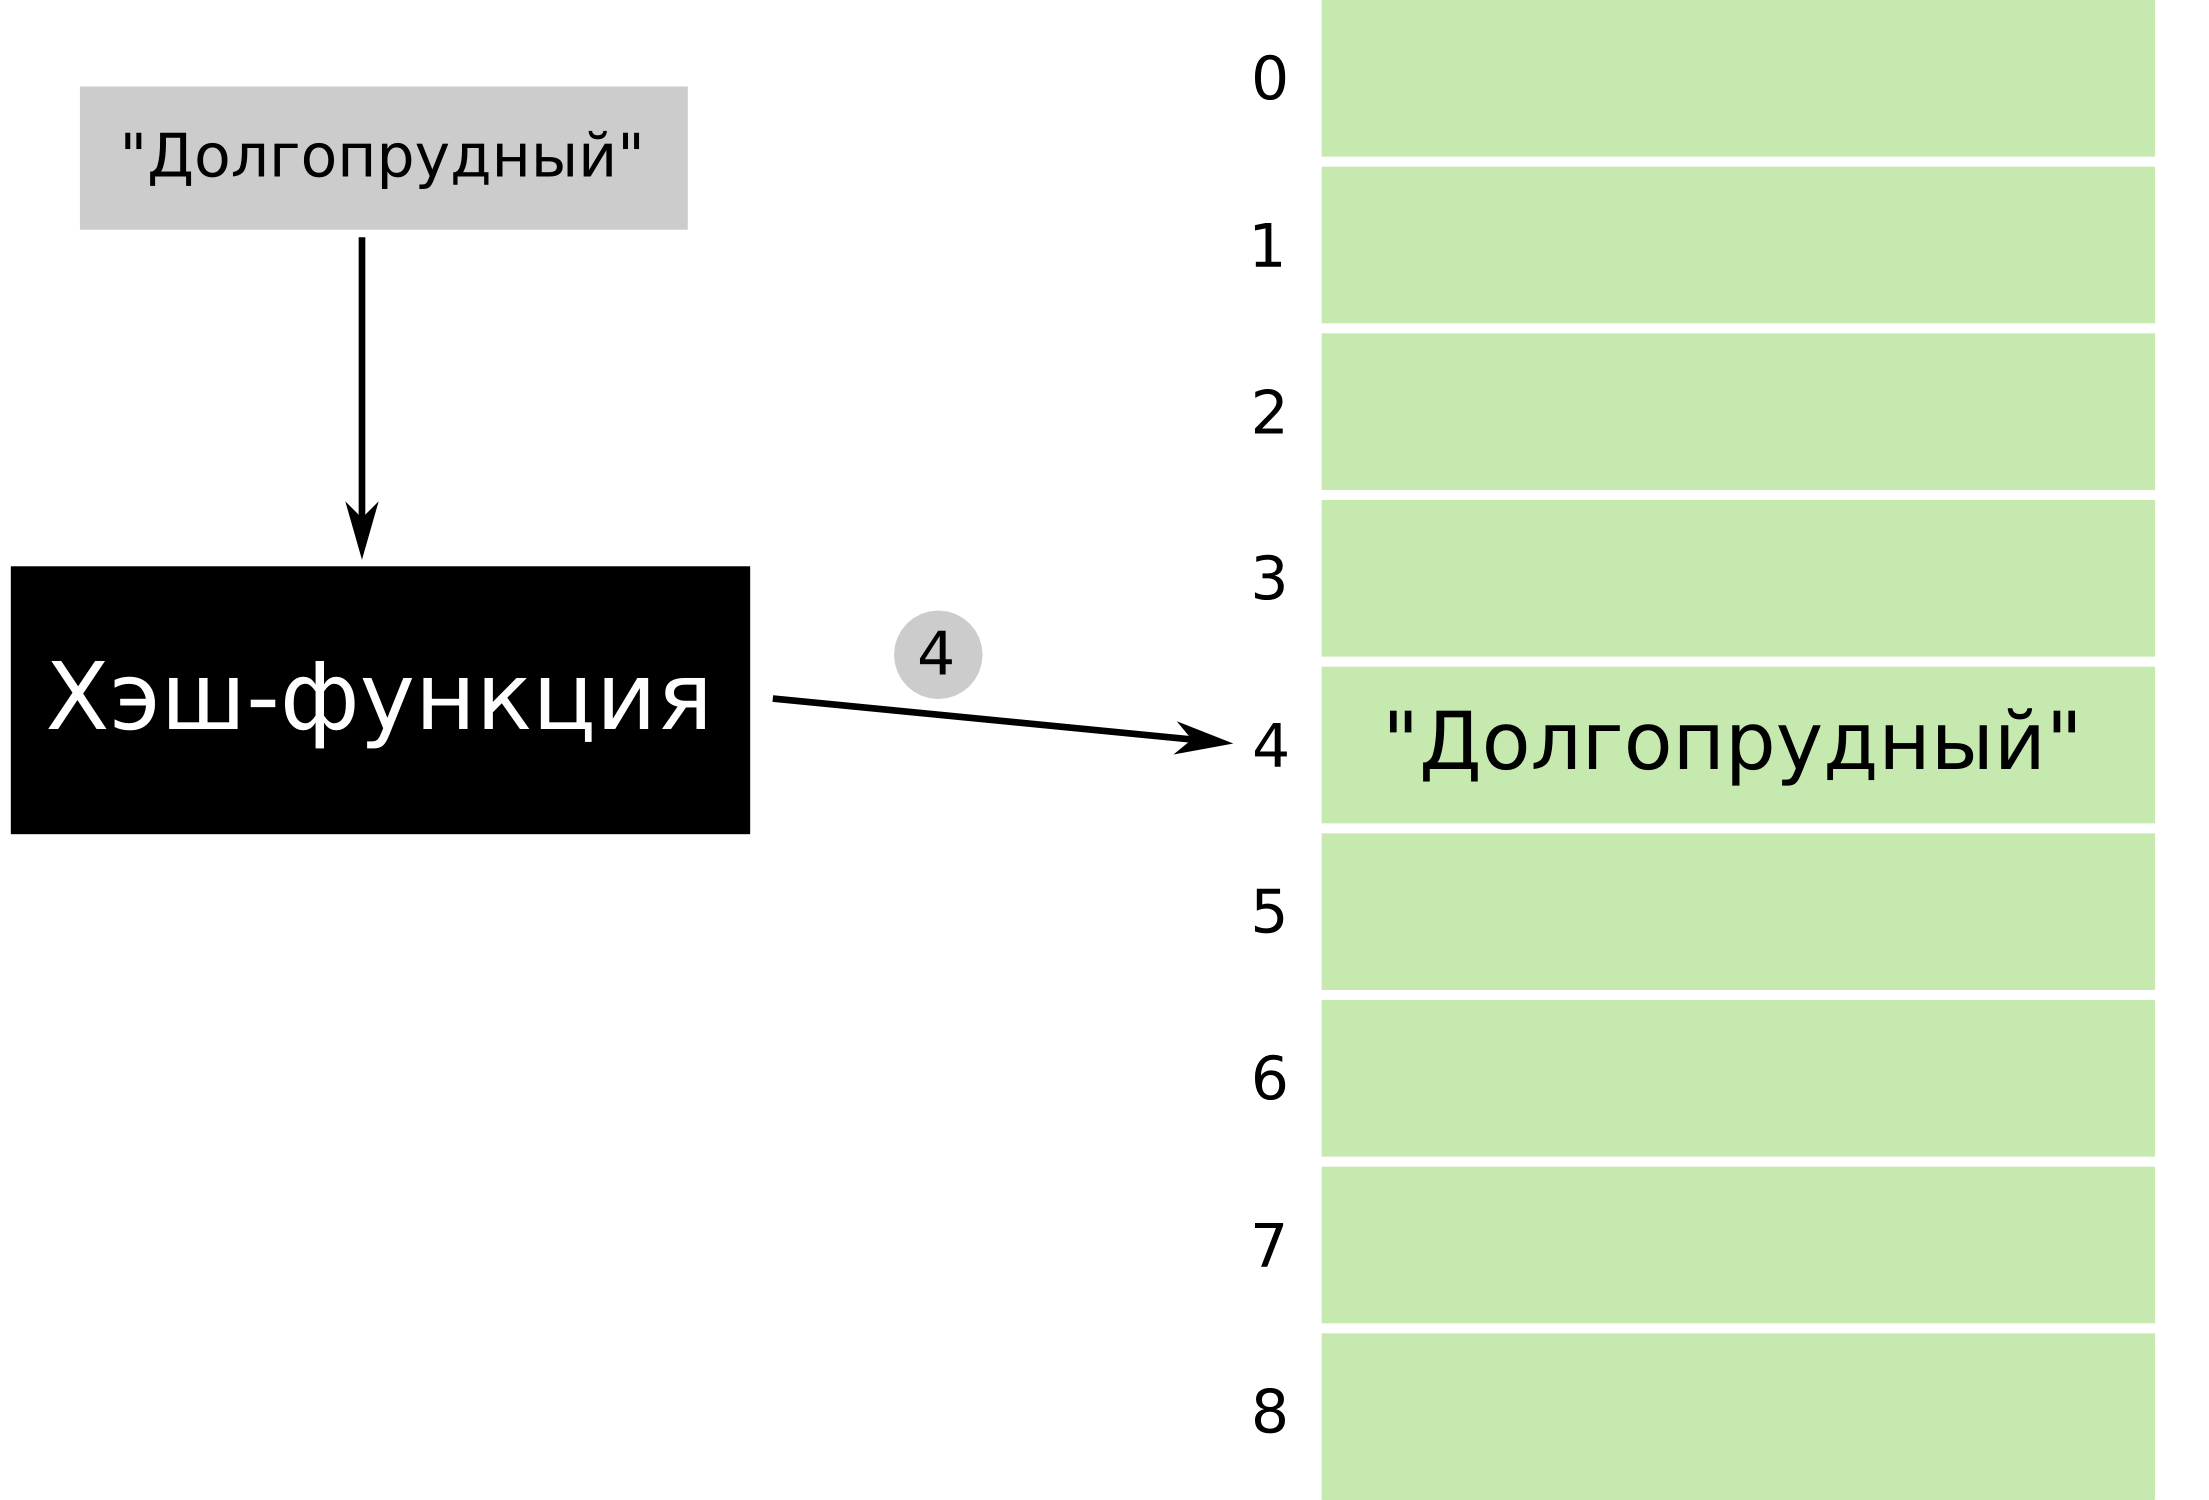
\includegraphics[width=0.86\linewidth]{images/hash_3.png}}
\end{figure}
\end{frame}

\begin{frame}{Хэш-таблица.}
\begin{figure}
\centerline{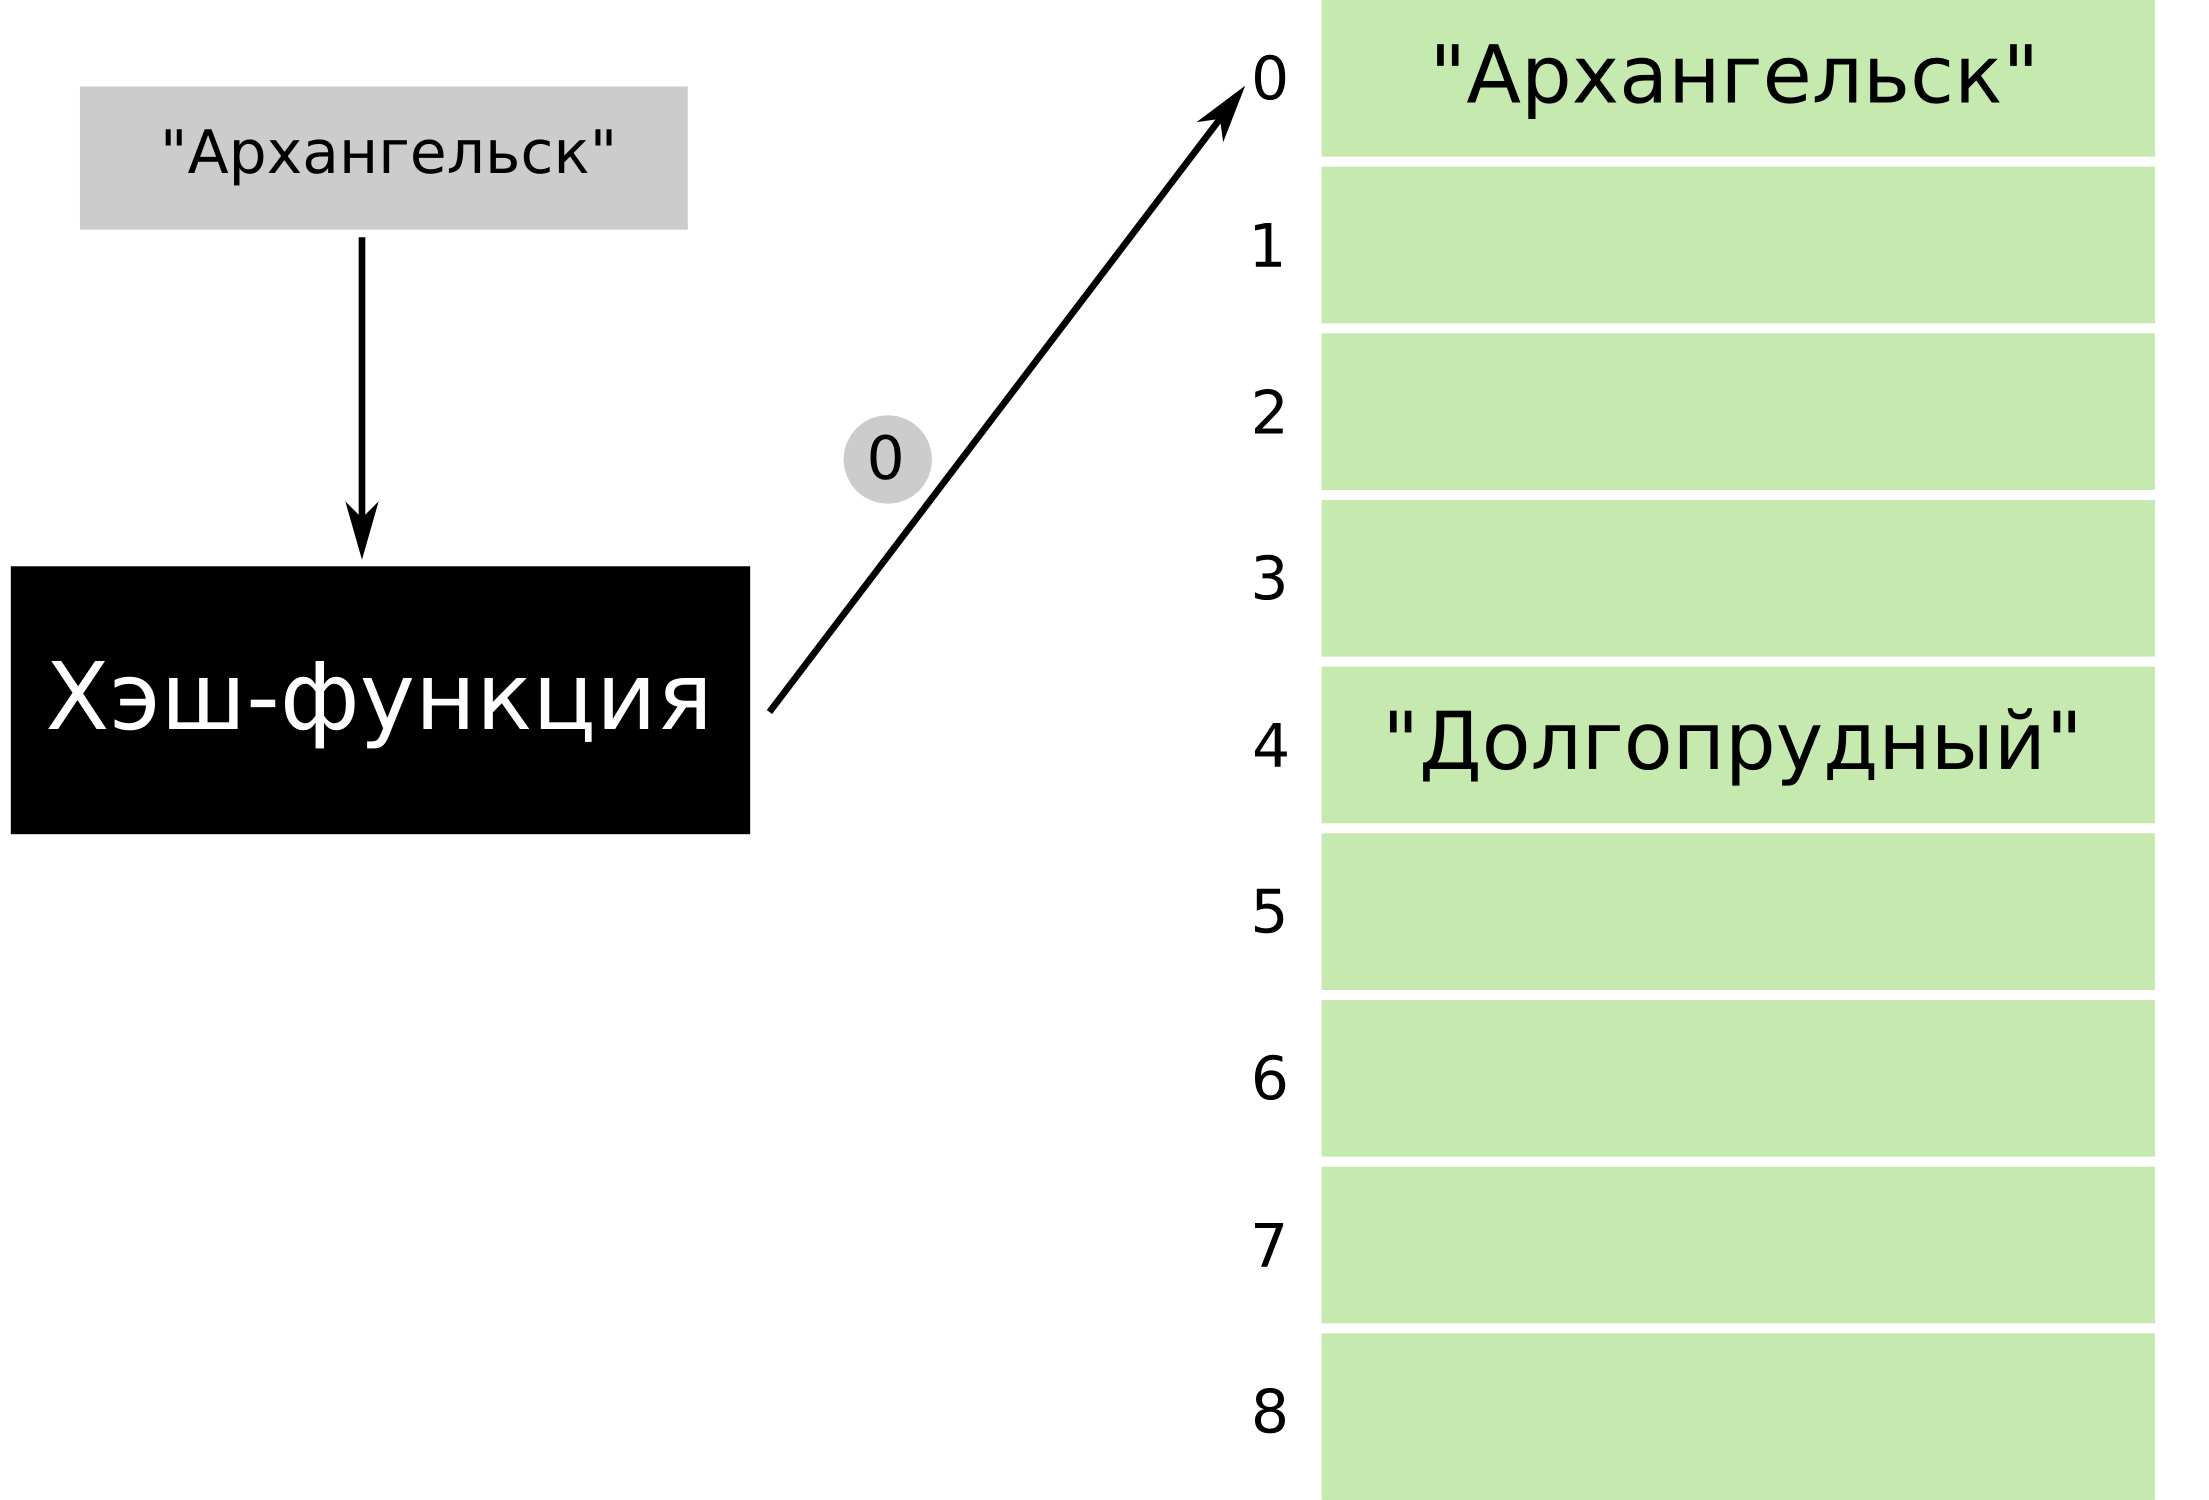
\includegraphics[width=0.86\linewidth]{images/hash_4.png}}
\end{figure}
\end{frame}

\begin{frame}{Хэш-таблица.}
\begin{figure}
\centerline{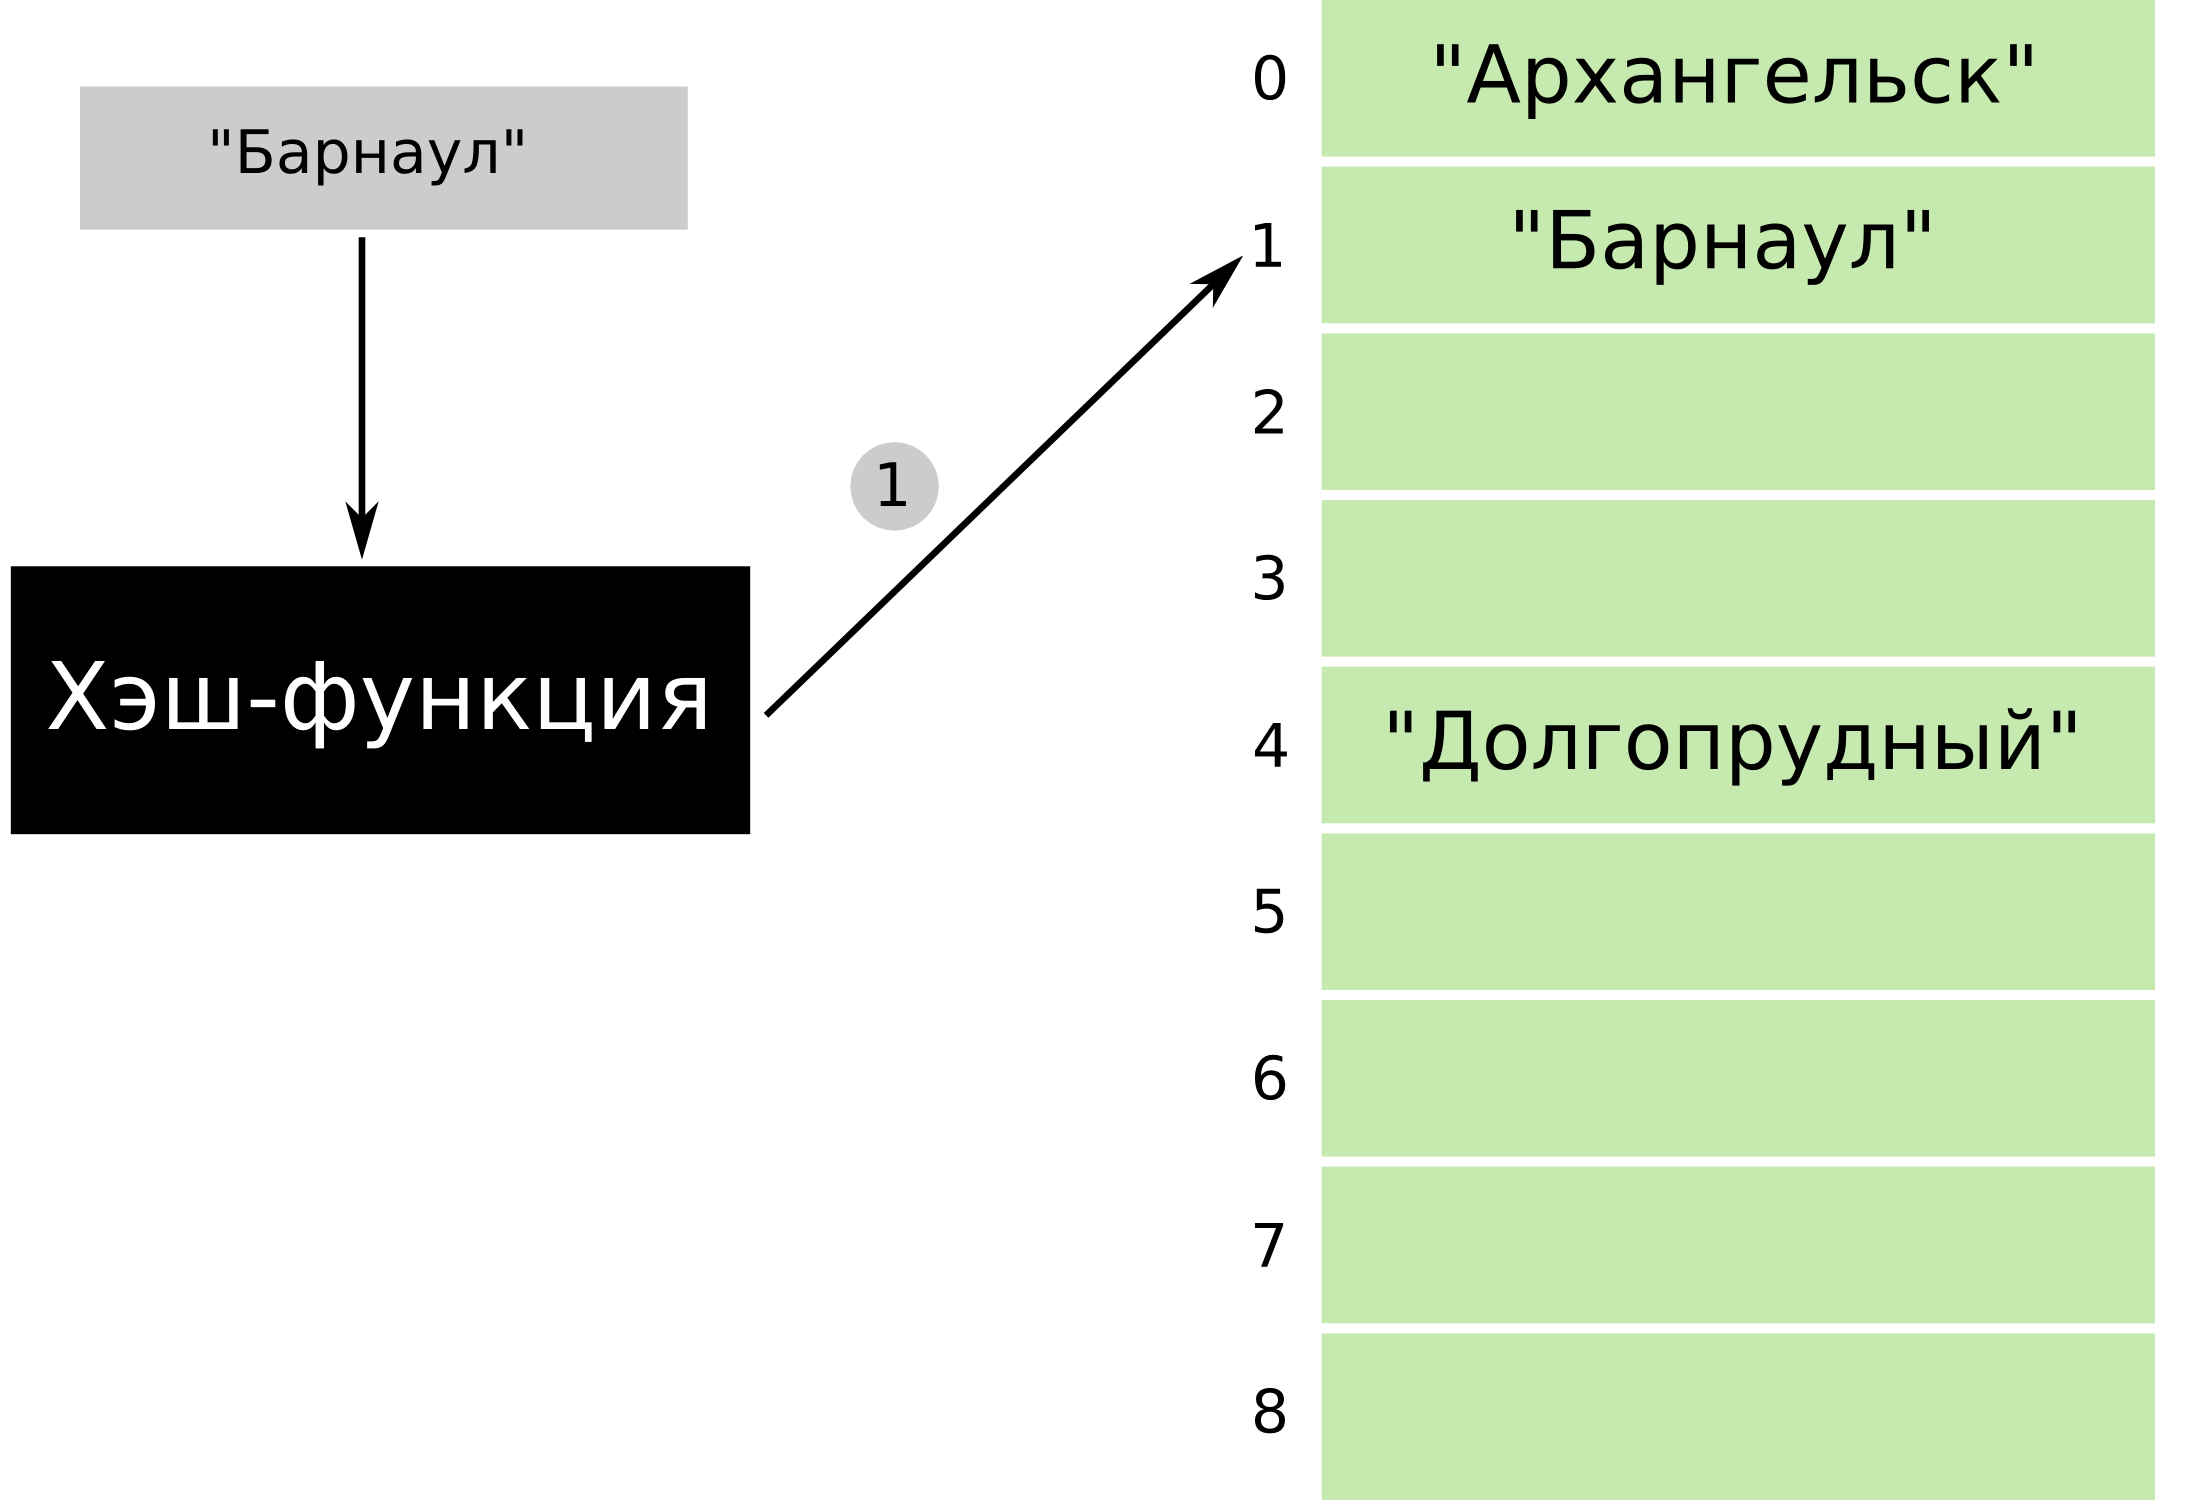
\includegraphics[width=0.86\linewidth]{images/hash_5.png}}
\end{figure}
\end{frame}

\begin{frame}{Хэш-таблица.}
\begin{figure}
\centerline{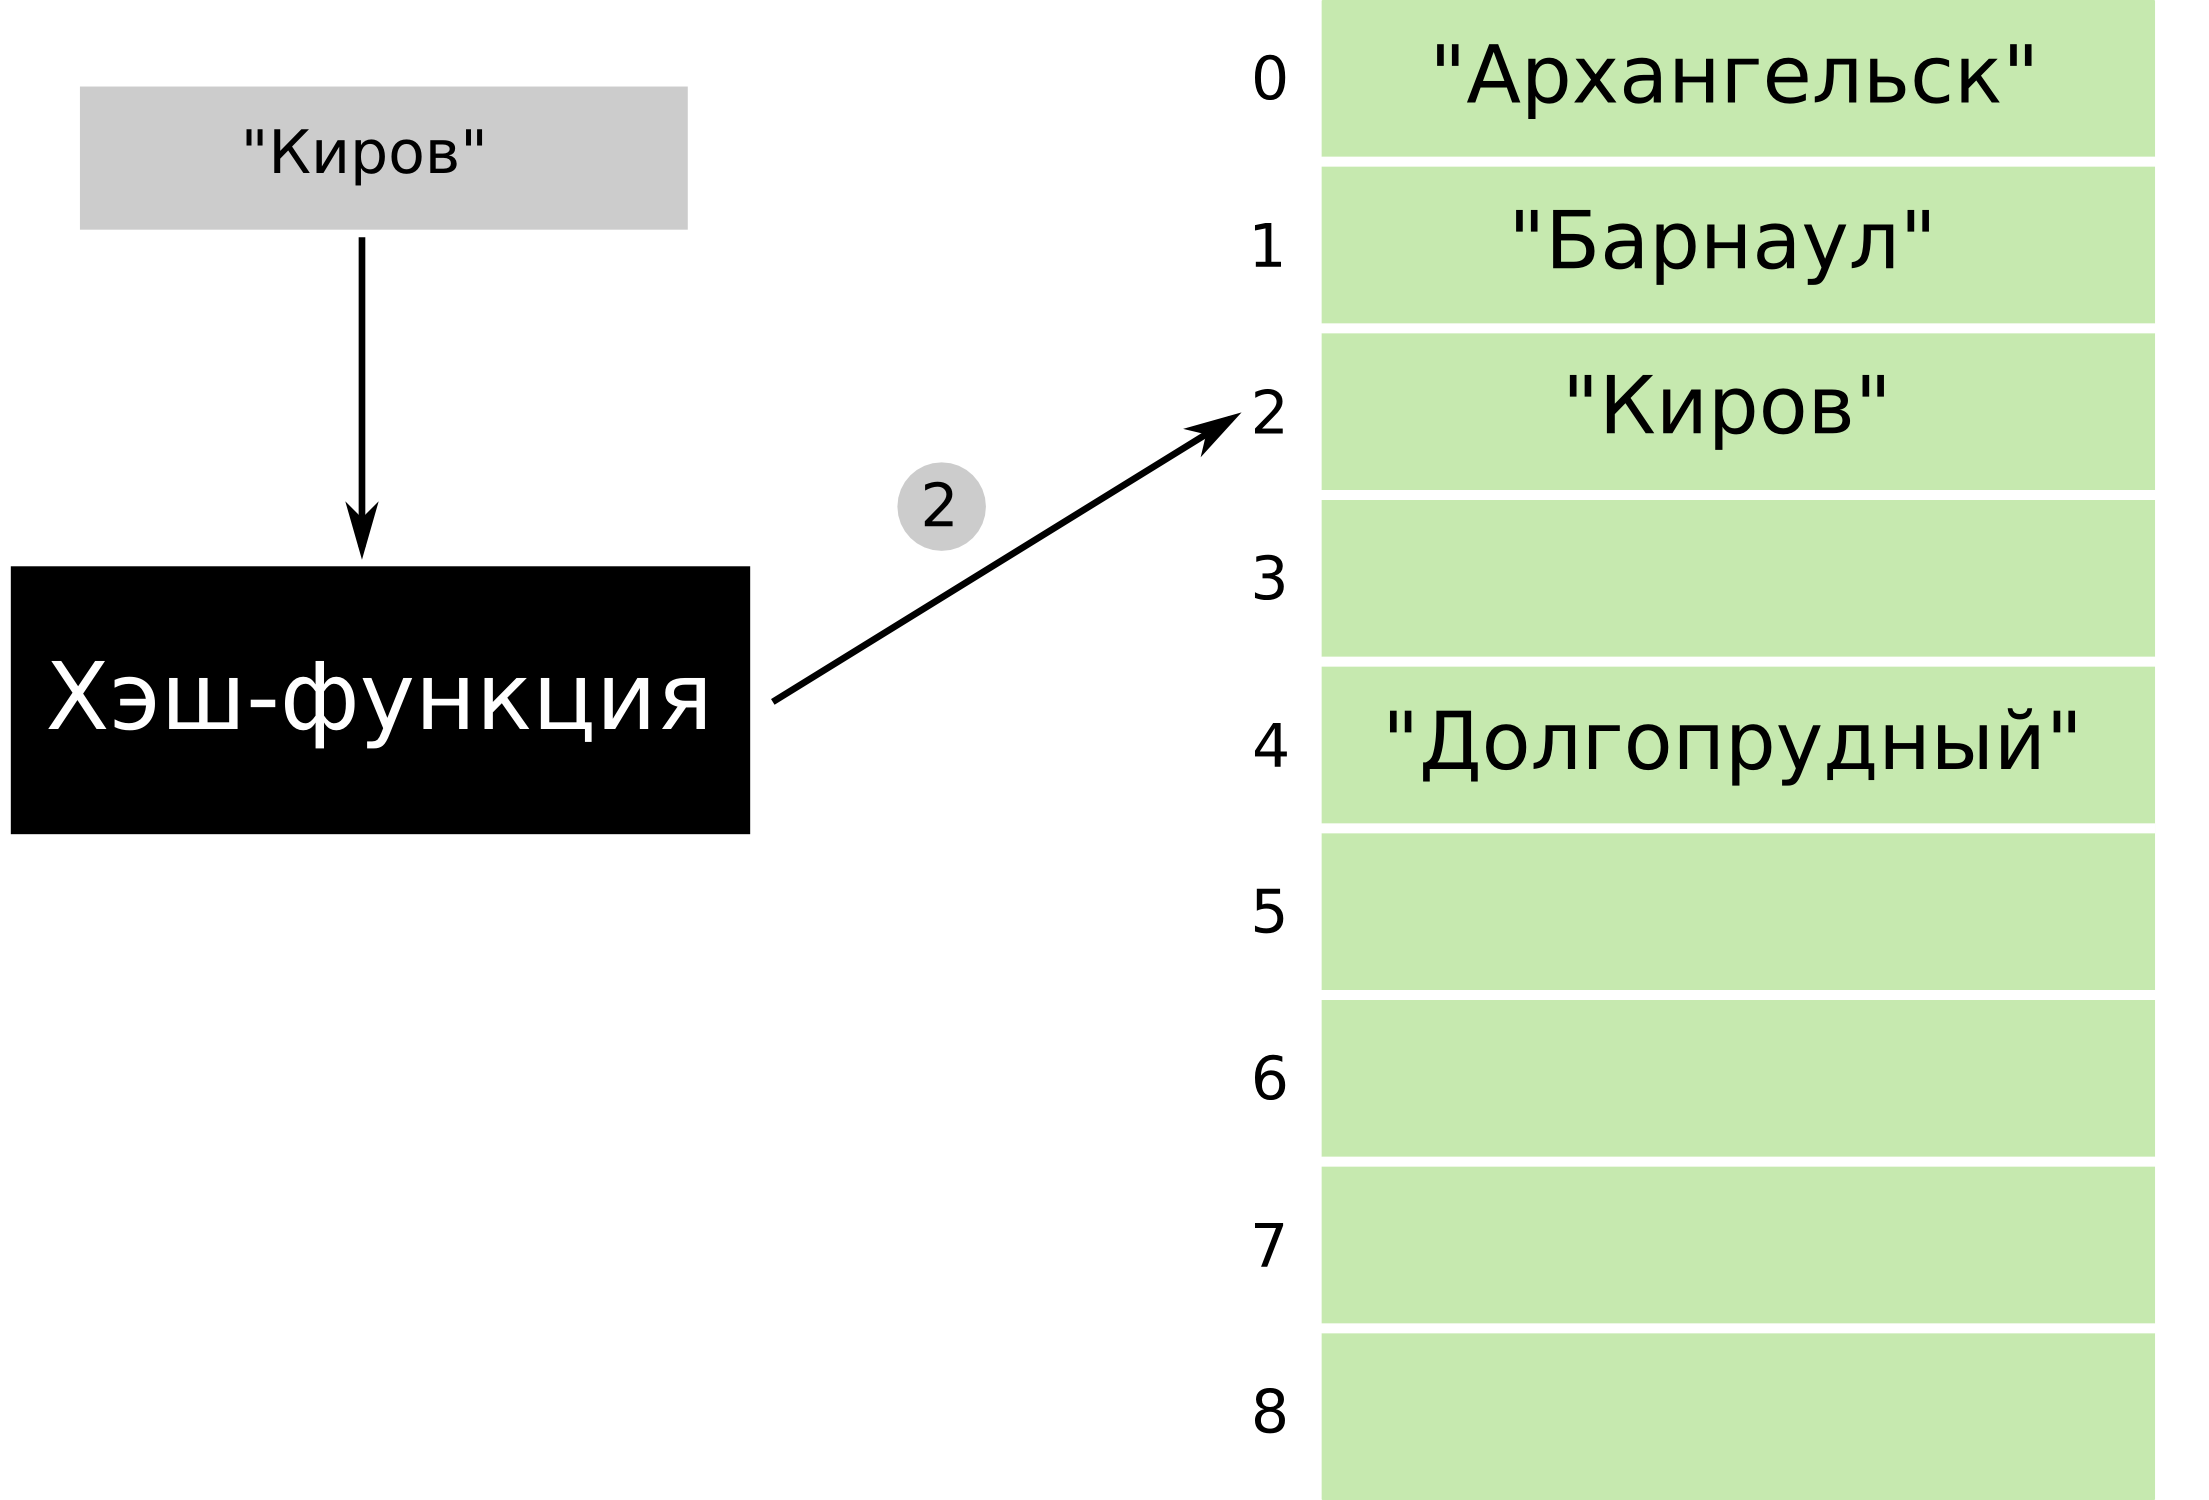
\includegraphics[width=0.86\linewidth]{images/hash_6.png}}
\end{figure}
\end{frame}

\begin{frame}{Хэш-таблица.}
\begin{figure}
\centerline{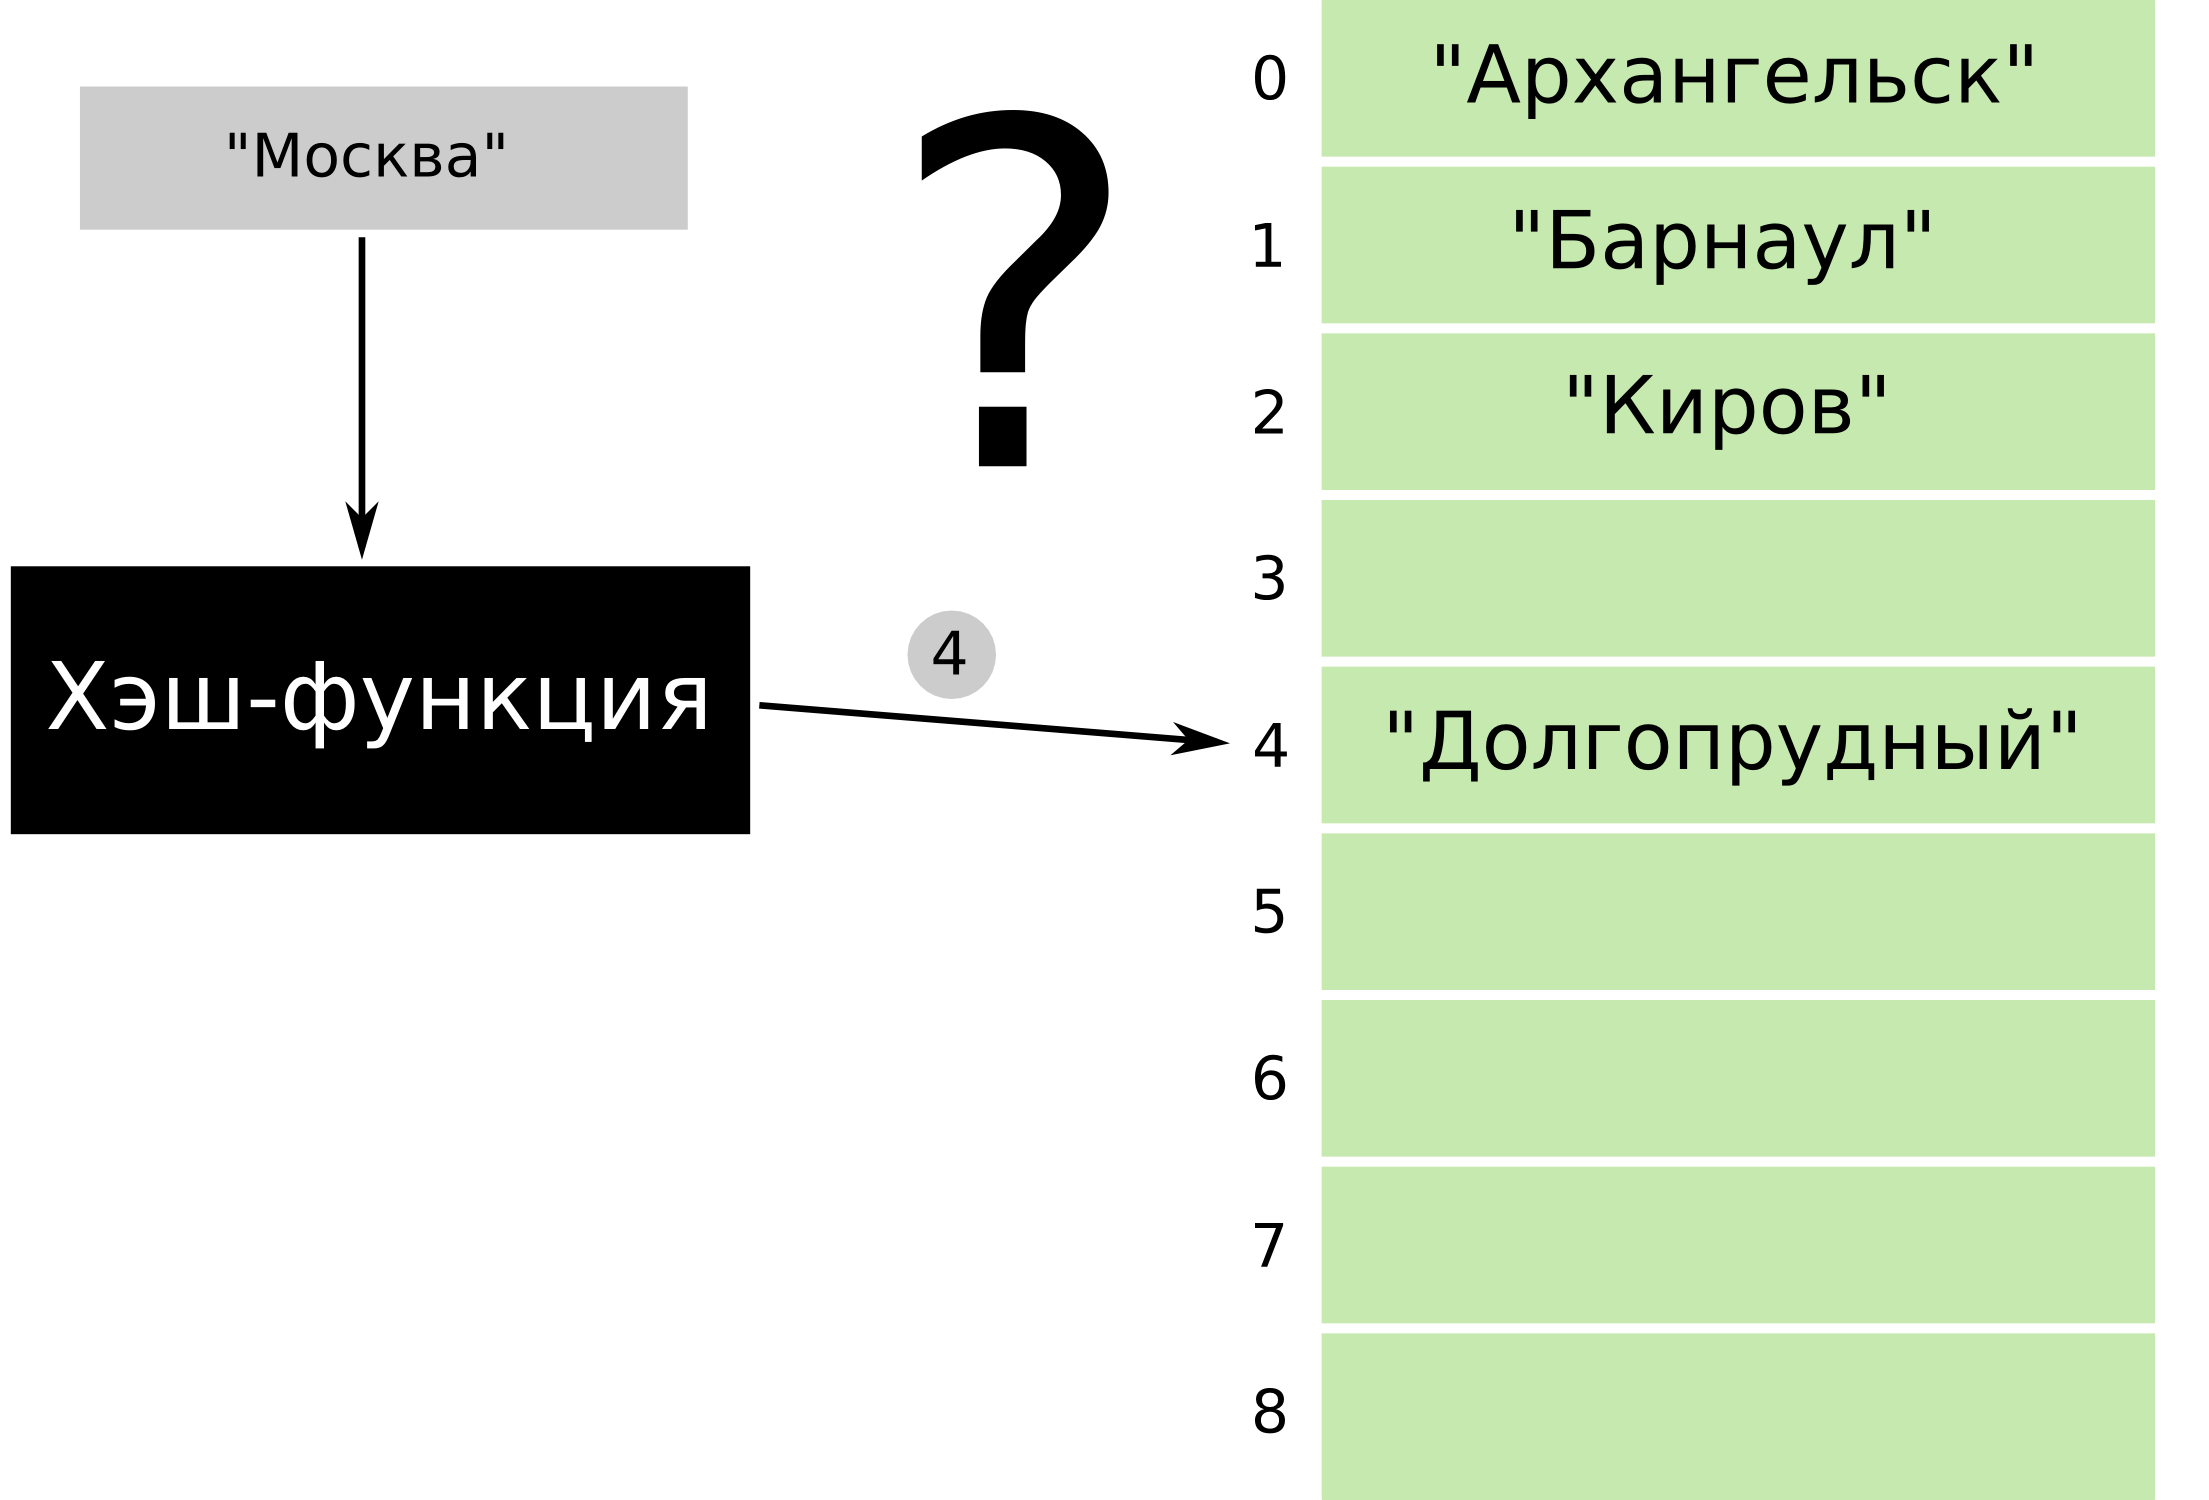
\includegraphics[width=0.9\linewidth]{images/hash_7.png}}
\end{figure}
\end{frame}

\begin{frame}{Хэш-таблица.}
\begin{figure}
\centerline{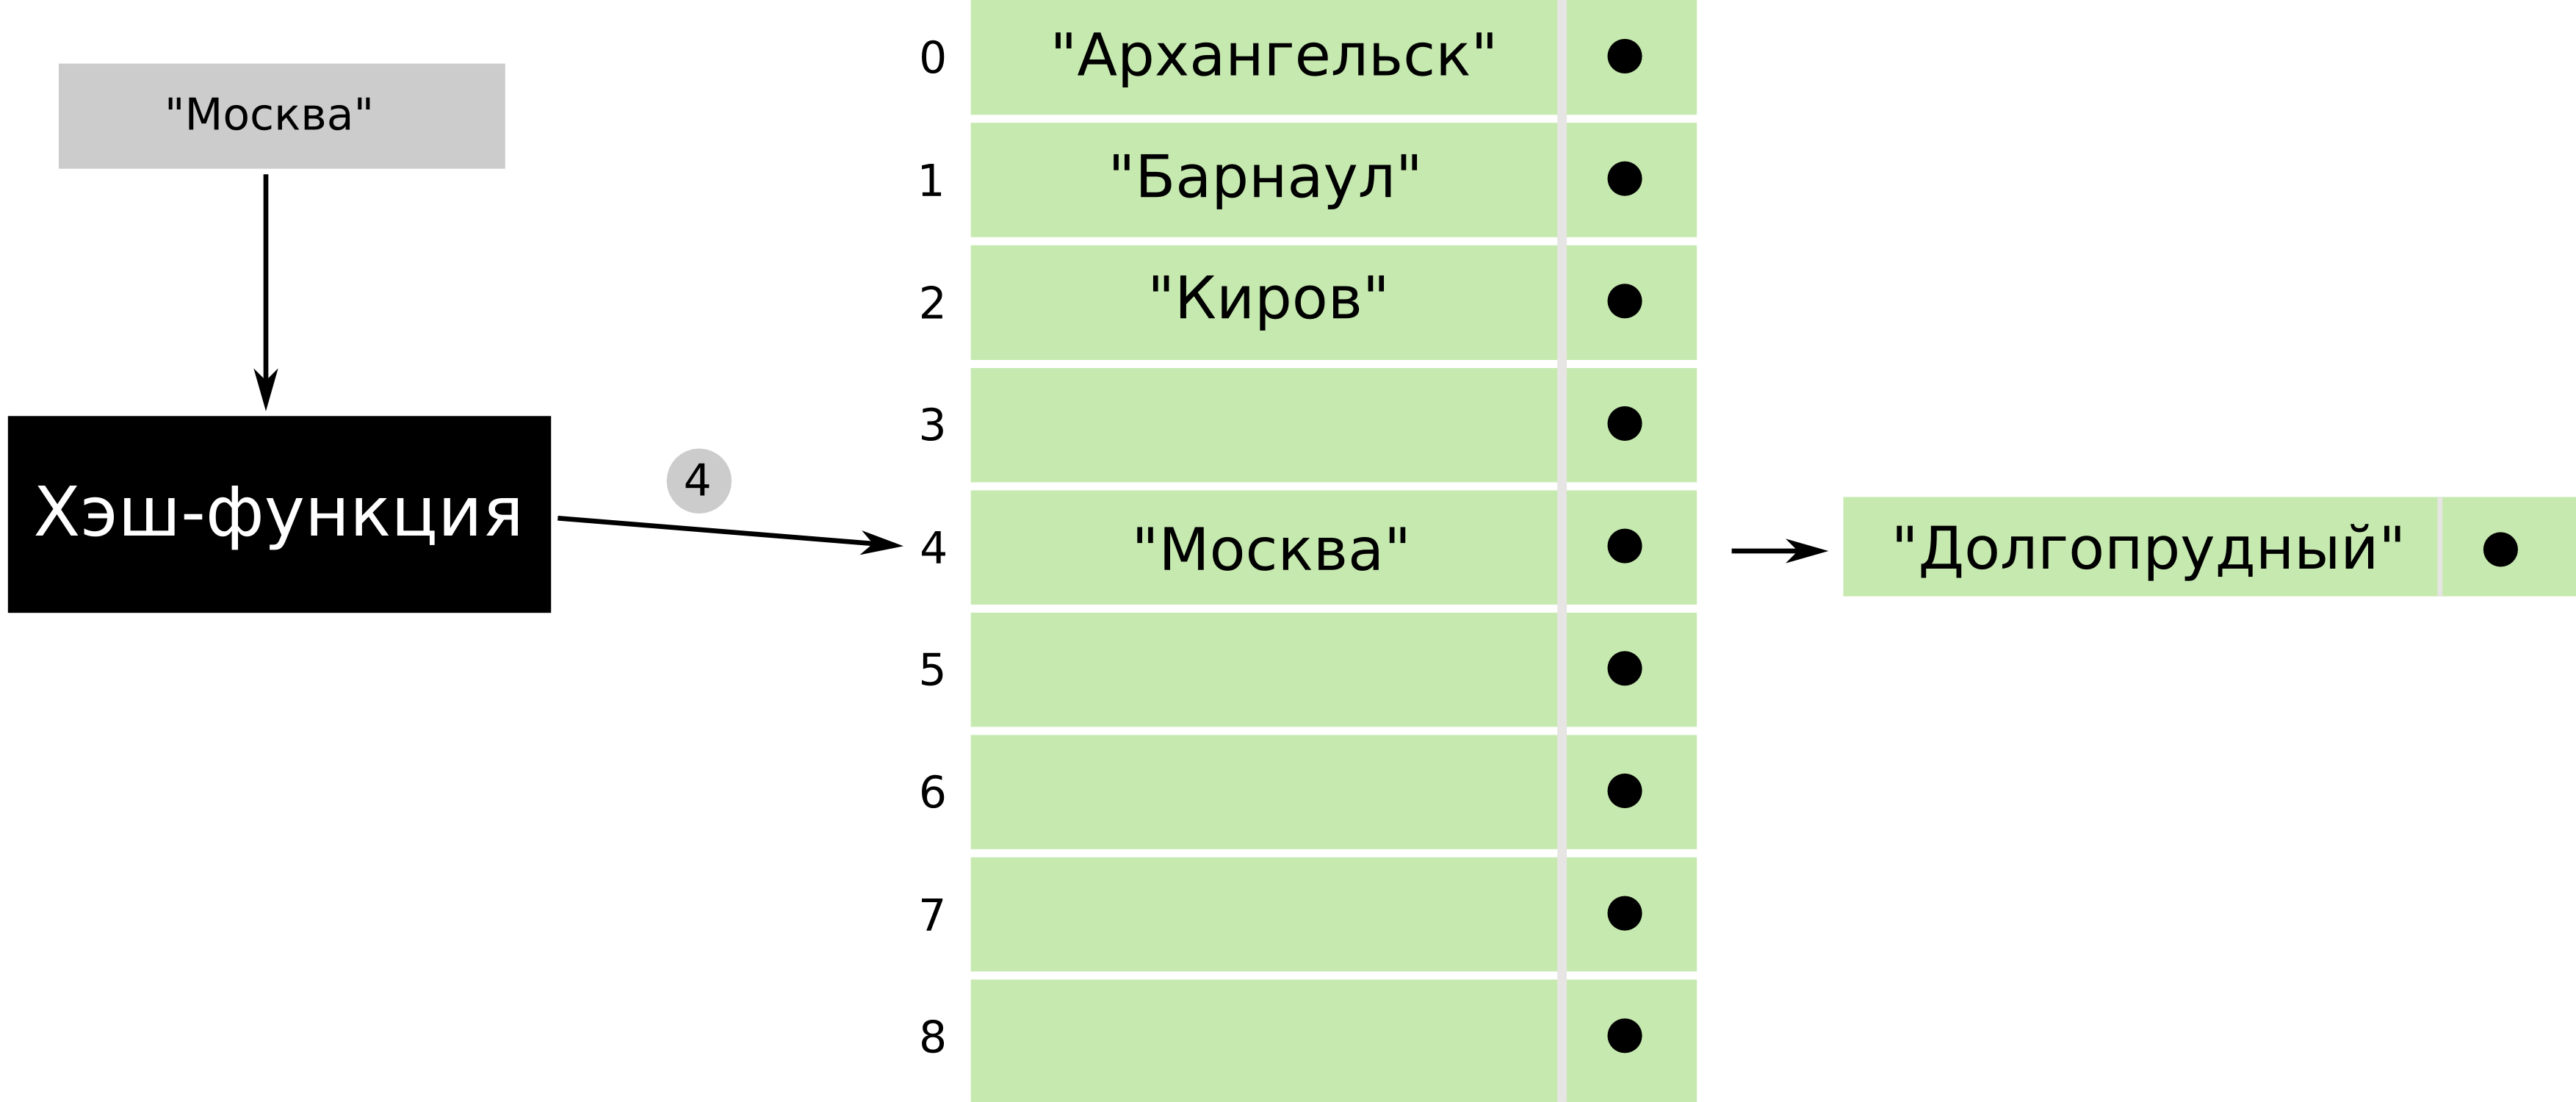
\includegraphics[width=0.99\linewidth]{images/hash_8.png}}
\end{figure}
\end{frame}

\begin{frame}{Хэш-таблица.}
\begin{figure}
\centerline{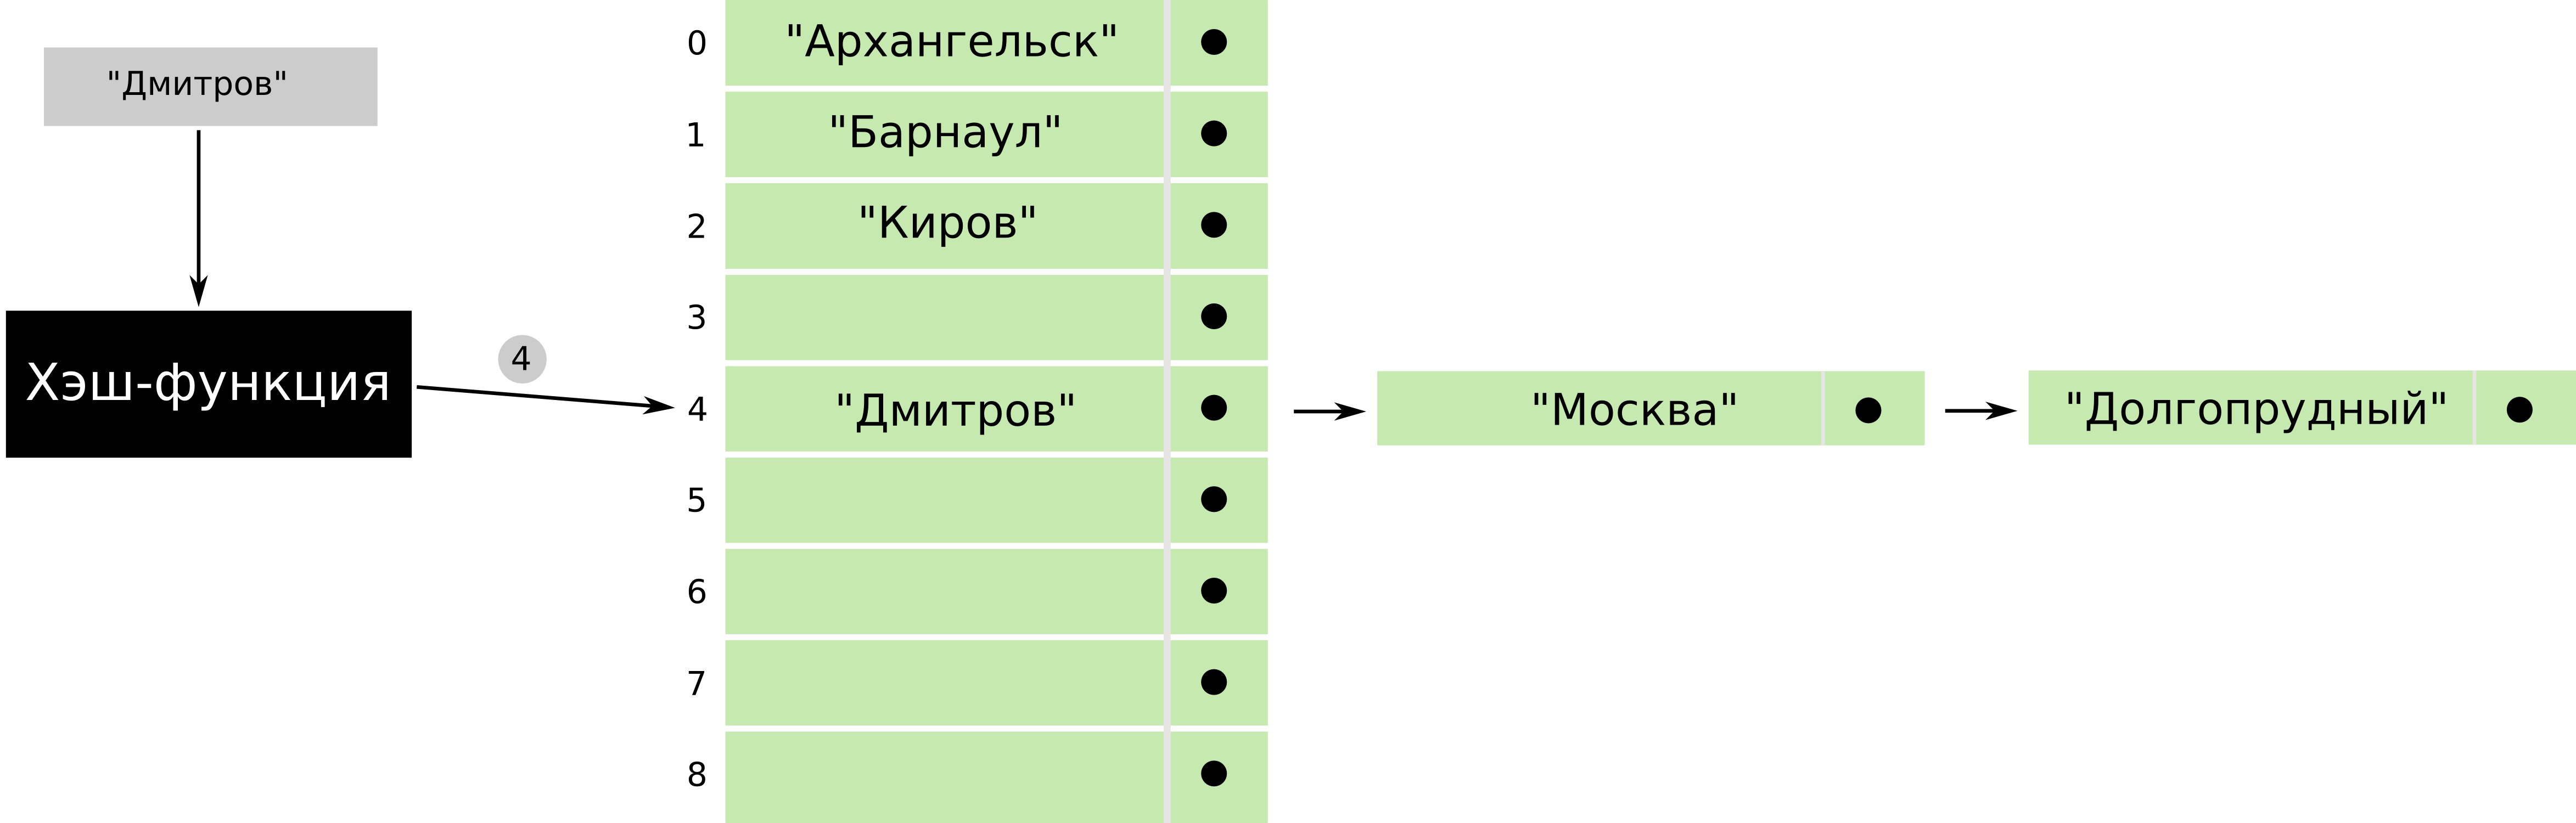
\includegraphics[width=0.99\linewidth]{images/hash_9.png}}
\end{figure}
\end{frame}


\begin{frame}{Свойства хорошей хэш-функции.}
\begin{itemize}
\item Работает быстро
\item Использует всю информацию, поступающую на вход
\item Значения на выходе хэш-функции распределены равномерномо
\item Похожие входные значения отображаются в существенно различные хэш-значения
\end{itemize}
\end{frame}


\section{Set и Map}

\begin{frame}{Абстрактный тип данных -- множество(Set)}
Реализация математического объекта множество:
$$
A = \{1, 4, 5\} \quad B = \{2, 4, 8, 9\}
$$
$$
A \cap B = \{4\} \quad A \cup B = \{1, 2, 4, 5, 8, 9\} \quad A \setminus B = \{1, 5\}
$$

Все эти операции есть и у множества -- абстрактного типа данных \\
Главное преемущество реализаций Set -- быстрые вставка, удаление и поиск (за O(1) в среднем; для реализации с помощью hash).
\end{frame}



\begin{frame}{Абстрактный тип данных -- словарь(associative array, map или dictionary )}
Абстрактный тип данных, позволяющий хранить пары вида «(ключ, значение)» и поддерживающий операции:
\begin{itemize}
\item INSERT(ключ, значение)
\item FIND(ключ)
\item REMOVE(ключ)
\end{itemize}
Все операции -- O(1) в среднем. \\
Удобно рассматривать как обычный массив, в котором в качестве индексов можно использовать не только целые числа, но и значения других типов — например, строки.
\end{frame}

%-=-=-=-=-=-=-=-=-=-=-=-=-=-=-=-=-=-=-=-=-=-=-=-=
%	Practical part:
%-=-=-=-=-=-=-=-=-=-=-=-=-=-=-=-=-=-=-=-=-=-=-=-=


\section{Практическая часть}






\end{document}